

GPS is the most ubiquitous localization system and generally
provides absolute coordinates. 
The usability of GPS in driving analytics has not been 
well discussed by the communities due to its high energy cost 
and coarse-grained measurements. 
Our measurements indicate GPS is a good 
candidate especially when IMU sensor
is not available to use or less accurate. 
We find that GPS has high accuracy in 
estimating speed and accelerations, 
especially in high speed scenarios (e.g., >10m/s).  
Given the simplicity of acceleration estimation
and high accuracy of GPS, 
we believe inertial sensors can be 
augmented by GPS in vehicle speed and acceleration
estimation applications. 




\nop{
Recently, Google announced that the raw data (e.g., pseudoranges, Dopplers and carrier phase) 
of GPS receiver is accessible for Android 7.0 \cite{android_gnss, google_gnss_tools}. 
}

\subsection{How GPS Works}

GPS provides a simple way to track vehicle motions
due to its orientation independent nature.
However, it has been blamed for its low
accuracy \cite{hedgecock2013high, gowda2016tracking}.
A GPS receiver can compute the instant absolute location
by receiving ephemeris data transmitted from satellite systems. 
The GPS satellites transmit signal with the starting 
time of the transmission (obtained from the satellites' atomic clock). 
Meanwhile, the ground receiver records the time of reception with 
smartphone local clock. 
The flight-time is the gap between these timestamps. 
The major error is caused by the smartphone GPS receiver
clock biases \cite{hedgecock2013high, gowda2016tracking}. 
Considering we are interested in the relative position of 
two continuous measurements from the same GPS receiver, 
the clock biases of the measurements are neutralized. 
In this work, we use smartphone built-in GPS as 
an augmenting method for driving analytics. 
We leave the performance gain by utilizing GPS raw data for the future work.


\subsection{Speed Estimation}

\begin{figure}[!htbp]
\begin{center}
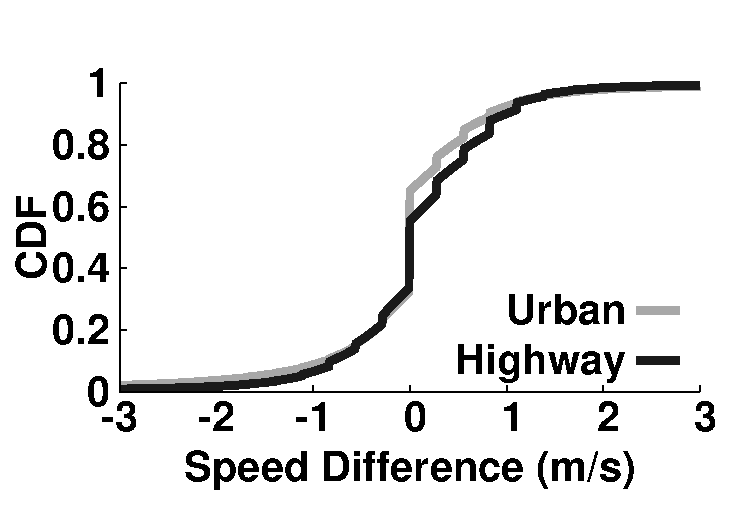
\includegraphics[width=2.6in,angle=0]{Figs/DriveSense/gpsobd_speed_diff.pdf}
\vspace{-0.2cm}
\caption{The speed estimation error of GPS.}
\vspace{-0.2cm}
\label{speeddiff}
\end{center}
\end{figure}

Speed calculation is very important for many vehicular applications \cite{hansenspeed, chandrasekaran2010vehicular}.  
GPS can provide speed information by simply calculating
the distance and time difference between two adjacent points. 
We use dataset $\#1$ (more details in section \ref{evaluation}) to evaluate the speed estimation of GPS. 
We tag the dataset with highway trips and urban trips,
based on speed distributions. 
Trips with a speed over $50mph$ in any segment is classified into highway trips. 
The CDF of speed estimation errors are plotted in Fig. \ref{speeddiff}. 
More than $90\%$ of the points are able to accurately calculate the speed 
with the error less than $1m/s$. 


\subsection{Acceleration Estimation}



\begin{figure}[!tb]
\begin{center}
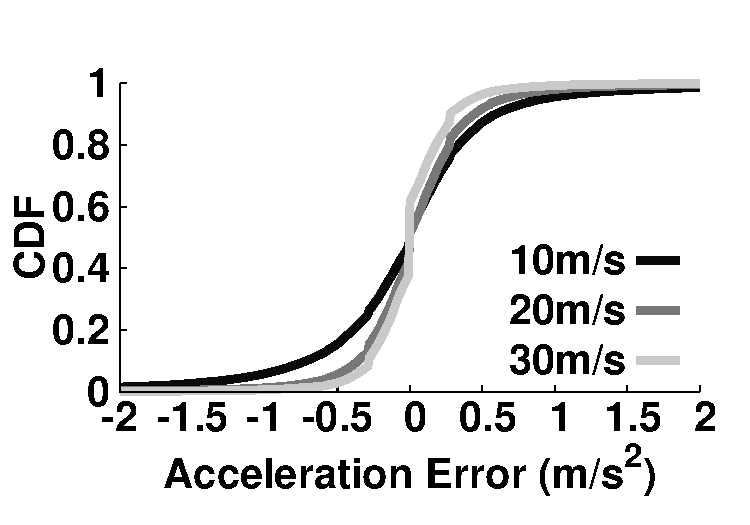
\includegraphics[width=3.0in,angle=0]{Figs/DriveSense/gpsobd_acce_speed.pdf}
\vspace{-0.2cm}
\caption{Acceleration estimation errors of GPS in urban and highway environments. 
	The estimation is more accurate in higher speed ($>10m/s$) than lower speed ($<10m/s$).}
\vspace{-0.2cm}
\label{accediff}
\end{center}
\end{figure}


The acceleration is comparatively evaluated by GPS points and OBD speed data.  
The CDF of estimation error is shown in Fig. \ref{accediff}. 
Each curve stands for the acceleration estimation error no more than that speed, i.e., 
$10m/s$ refers to any speeds not higher than $10m/s$ and $20m/s$ refers to any speeds between $10m/s$ and $20m/s$. 
The estimation errors of GPS in low speed are caused by GPS location estimation errors, which could be caused by either the weak GPS satellite signal or strong thermo-noise floor. 
Additionally, the errors could also be caused by the building and vehicle blockage.  
The acceleration estimation when the vehicular speed is higher than $20m/s$ 
is highly accurate. 
This result indicates that GPS is more accurate in high speed scenarios.




\subsection{GPS Availability}



\begin{figure}[!tb]
\begin{center}
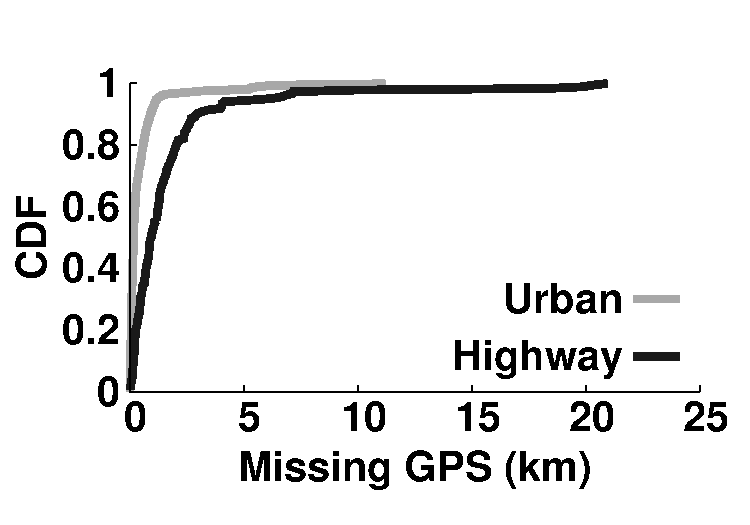
\includegraphics[width=1.7in,angle=0]{Figs/DriveSense/missing_gps.pdf}
\hspace{-0.5cm}
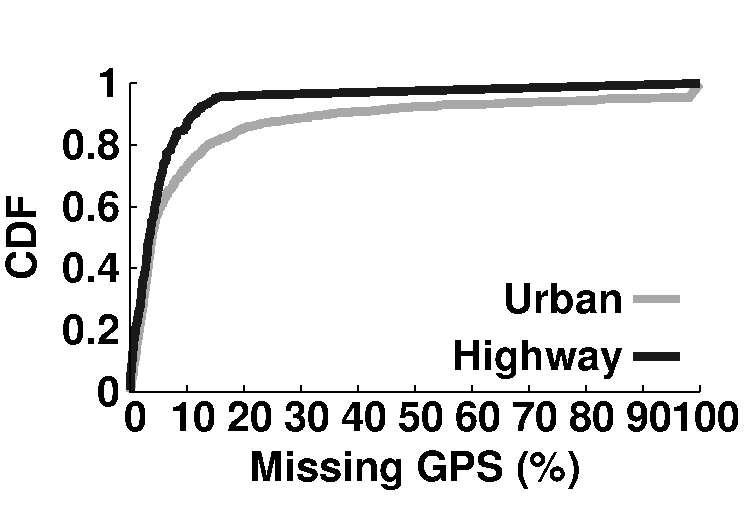
\includegraphics[width=1.7in,angle=0]{Figs/DriveSense/missing_percent.pdf}
\vspace{-0.2cm}
\caption{GPS availability in urban and highway environments. }
\vspace{-0.2cm}
\label{missinggps}
\end{center}
\end{figure}


GPS signal is not always available, especially in indoor
environments.
If the smartphone is inside the car, there are chances
that the smartphone GPS receiver is not able 
to detect satellite signals.  
Also, if the car is passing through underground tunnel or high buildings, 
GPS signal might be too weak to be received. 
We compare GPS and OBD data point by point, 
and record the accumulated distance of trip fragment without GPS points. 
The missing GPS of each trip is illustrated in Fig. \ref{missinggps}. 
There are a couple of trips that are entirely missing, 
while we are not sure if it is caused by software bugs or blocked signals. 
The GPS is available most of the time, while there are cases
that the GPS is missing at the start and/or end of the trip. 




 


%%%%%%%%%%%%%%%%%%%%%%%%%%%%%%%

\nop{
\subsection{Steering Angle Estimation}

\begin{figure}[!htbp]
\begin{center}
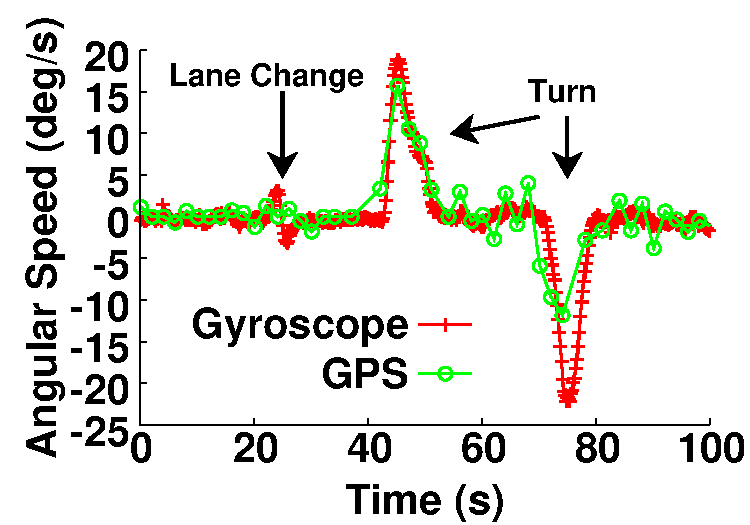
\includegraphics[width=2.6in,angle=0]{Figs/DriveSense/angular_illustration.pdf}
\vspace{-0.2cm}
\caption{An illustration of steering angular velocity estimation of GPS.}
\vspace{-0.2cm}
\label{steeringillustration}
\end{center}
\end{figure}

\begin{figure}[!htbp]
\begin{center}
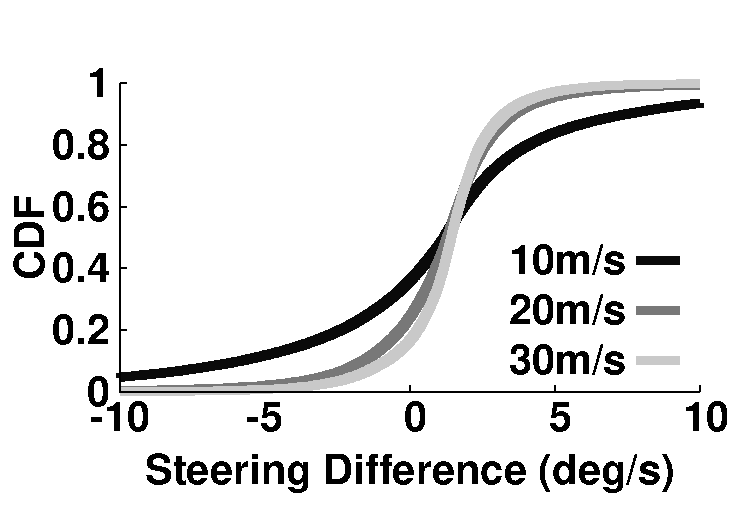
\includegraphics[width=2.6in,angle=0]{Figs/DriveSense/gps_steering.pdf}
\vspace{-0.2cm}
\caption{The GPS steering angular velocity estimation difference comparing with gyroscope.}
\vspace{-0.2cm}
\label{steeringdiff}
\end{center}
\end{figure}

Another important aspect of vehicle motion is steering motion. 
GPS can be used to estimate the changes of steering angle
by using a two pass processing. 
The first pass is used to calculate the moving direction
based on two GPS point. 
The second pass is used to calculate the angular attitude
rate based on direction differences. 
There are more noises on GPS readings
in low speed, i.e., the GPS indicates the vehicle is 
moving while the car is actually not, or the vehicle is stable but the GPS indicate the movement. 
Using adjacent points to calculate the direction introduces
lots of noises. 
We use the next GPS point at least $l-meter$ 
away as the next hop to calculate the direction. 
We compare the angular attitude rate estimated by GPS with
the ones estimated by 
gyroscope.
A trip fragment is illustrated in Fig.\ref{steeringillustration}
and the statistics are plotted in Fig. \ref{steeringdiff}.
Three observations can be concluded from this two Figs/DriveSense. 
First, the steering angular velocity estimated by GPS
is very coarse-grain, and cannot be used
for small direction movement such as lane changes. 
To detect the lane change, a precision of $0.5deg/s$ 
is required, while more than $80\%$ of the 
estimation error (by GPS) is higher than $1deg/s$.
Second, GPS can be used to identify large direction
changes such as turns, e.g., GPS can detect $83.54\%$
of the turns detected by gyroscope. 
GPS is very noisy when steering around parking lot
and cannot used for motion detection. 
Third, similar to acceleration estimation, 
the estimation accuracy of angular velocity is higher 
in high speed scenarios. 
}


